\def\documentauthor{Carlos Salinas}
\def\hwnum{4}
\def\documenttitle{MA166: Recitation {\hwnum} Script}
\def\shorttitle{MA166-Recitation-{\hwnum}-Script}
\def\coursename{MA166}
\def\documentsubject{calculus ii}
\def\authoremail{salinac@purdue.edu}

\documentclass[article,oneside,10pt]{memoir}
\usepackage{geometry}
\usepackage[dvipsnames]{xcolor}

\usepackage[
    breaklinks,
    bookmarks=true,
    % colorlinks=true,
    pageanchor=false,
    linkcolor=black,
    anchorcolor=black,
    citecolor=black,
    filecolor=black,
    menucolor=black,
    runcolor=black,
    urlcolor=black,
    hyperindex=false,
    hyperfootnotes=true,
    pdftitle={\shorttitle},
    pdfauthor={\documentauthor},
    pdfkeywords={\documentsubject},
    pdfsubject={\coursename}
    ]{hyperref}

% Use symbols instead of numbers
\renewcommand*{\thefootnote}{\fnsymbol{footnote}}

%% Math
\usepackage{bm}
\usepackage{amsmath}
\usepackage{amssymb}
\usepackage{amsthm}
\usepackage{mathtools}
\usepackage[mathcal]{euscript}
\usepackage{mathrsfs}
\usepackage{wasysym}

\usepackage[LAE,LFE,T2A,T1]{fontenc}
\usepackage[utf8]{inputenc}
\usepackage[farsi,french,german,spanish,russian,english]{babel}
\babeltags{fr=french,
           de=german,
           en=english,
           es=spanish,
           pa=farsi,
           ru=russian
           }
\def\spanishoptions{mexico}

\selectlanguage{english}

\newcommand{\textfa}[1]{\beginR\textpa{#1}\endR}

\usepackage{cmap}
\usepackage{CJKutf8}
\newcommand{\textkr}[1]{\begin{CJK}{UTF8}{mj}#1\end{CJK}}
\newcommand{\textjp}[1]{\begin{CJK}{UTF8}{min}#1\end{CJK}}
\newcommand{\textzh}[1]{\begin{CJK}{UTF8}{bsmi}#1\end{CJK}}

\usepackage{graphicx}
\graphicspath{{figures/}}

% Misc
\usepackage{microtype}
\usepackage{soul}
\usepackage{multicol}
\usepackage[inline]{enumitem}
\usepackage{listings}
\usepackage{mleftright}
\mleftright

\usepackage{siunitx}

%% Theorems and definitions
%% remove parentheses
% \makeatletter
% \def\thmhead@plain#1#2#3{%
%   \thmname{#1}\thmnumber{\@ifnotempty{#1}{ }\@upn{#2}}%
%   \thmnote{ {\the\thm@notefont#3}}}
% \let\thmhead\thmhead@plain
% \makeatother

\theoremstyle{plain}
\newtheorem{theorem}{Theorem}
\newtheorem{proposition}[theorem]{Proposition}
\newtheorem{corollary}[theorem]{Corollary}
\newtheorem{claim}[theorem]{Claim}
\newtheorem{lemma}[theorem]{Lemma}
\newtheorem{axiom}[theorem]{Axiom}

\newtheorem*{corollary*}{Corollary}
\newtheorem*{claim*}{Claim}
\newtheorem*{lemma*}{Lemma}
\newtheorem*{proposition*}{Proposition}
\newtheorem*{theorem*}{Theorem}

\theoremstyle{definition}
\newtheorem{definition}{Definition}
\newtheorem{example}{Examples}
\newtheorem{examples}[example]{Examples}
\newtheorem{exercise}{Exercise}[chapter]
\newtheorem{problem}[exercise]{Problem}

\newtheorem*{example*}{Example}
\newtheorem*{exercise*}{Exercise}
\newtheorem*{problem*}{Problem}

%% Redefinitions & commands
\newcommand{\nle}{\ensuremath{\not<}}
\newcommand{\nge}{\ensuremath{\not>}}
\newcommand{\nsubset}{\ensuremath{\not\subset}}
\newcommand{\nsupset}{\ensuremath{\not\supset}}
\newcommand\minus{\ensuremath{\null\smallsetminus}}
\renewcommand\qedsymbol{\ensuremath{\null\hfill\smiley{}}}

%% Commands and operators
\DeclareMathOperator{\comp}{comp}
\DeclareMathOperator{\proj}{proj}

\newcommand{\diff}{\,\mathrm{r}}

\newcommand{\bbC}{\mathbb{C}}
\newcommand{\bbN}{\mathbb{N}}
\newcommand{\bbQ}{\mathbb{Q}}
\newcommand{\bbR}{\mathbb{R}}
\newcommand{\bbZ}{\mathbb{Z}}

\newcommand{\bfu}{\mathbf{u}}
\newcommand{\bfv}{\mathbf{v}}
\newcommand{\bfw}{\mathbf{w}}

\begin{document}
\author{\href{mailto:\authoremail}{\documentauthor}}
\title{\documenttitle}
\date{\today}
\maketitle
\chapter{Script for Recitation 4}

\chapter{Exam Problems}
\begin{problem}[Fall 2015, \# 6]
The base of a solid is a circular disc in the $xy$-plane of radius
$1$. Its cross sections perpendicular to the $x$–axis are isosceles
right triangles, with hypotenuse in the base. Find the volume of this
solid.
\end{problem}
\begin{proof}[Solution]
We need a few equations to set this problem up. First, we need to find the
base, height, and area of a right isosceles triangle. Since two of the
sides of the isosceles triangle are the same and the angle between them is
$\pi/2$, by the Pythagorean theorem we have
\begin{equation}
\label{eq:base-height-of-isosceles}
b^2+h^2=b^2+b^2=2b^2={h'}^2
\end{equation}
where $b$ is the base, $h$ is the height (which in this case is equal to
the base $b$), and $h'$ is the hypotenuse. Then $b=h=h'/\sqrt{2}$. Hence,
the area of the triangle is
\begin{equation}
  \label{eq:area-of-isosceles-triangle}
\tfrac{1}{2}bh=\frac{1}{2}\left(\frac{{h'}^2}{2}\right)=\tfrac{1}{4}{h'}^2.
\end{equation}
Exploiting the geometry of the base, let us consider the right \ul{half}
of the circular base, find the area, and double our result to get the total
area. Now, how does the hypotenuse change of the isosceles triangle
changes as we move from left to right on the interval $0\leq x\leq 1$. At
$x=0$, the base of the hypotenuse will be $2$. If we move a little to the
right $x$, the hypotenuse will be given by the equation
\[
{h'}=2\sqrt{1-x^2}.
\]
Then, plugging in this value into our equation for the area (Equation
(\ref{eq:area-of-isosceles-triangle})) we have
\[
\tfrac{1}{4}{h'}^2=\tfrac{1}{4}\left(2\sqrt{1-x^2}\right)^2=1-x^2.
\]
Now, approximating the volume by the Riemann sum and taking the limit, we
get the volume over $0\leq x\leq 1$
\[
\int_0^1 1-x^2\diff x=\left.x-\tfrac{1}{3}x^3\right|_0^1=1-\frac{1}{3}=\frac{2}{3}.
\]
Last but not least, let us double the volume to get a total of
\[
V=2\left(\frac{2}{3}\right)=\boxed{\frac{4}{3}.}
\]
\end{proof}

\chapter{Homework 8 Solutions}
% p449:3,5,7,10,19,21
\begin{problem}[WebAssign, HW8, 1]
  A variable force of $2x^{-2}$ pounds moves an object along a straight
  line when it is $x$ feet from the origin. Calculate the work done in
  moving the object from $x=1$ ft to $x=15$ ft. (Round your answer to two
  decimal places.)
\end{problem}
\begin{proof}[Solution]
Recall the formula for the work done by a fore as a function of distance?
It is given by
\[
W=\int_1^15 F(x)\diff x=
2\int_1^{15} x^{-2}\diff x=
-2\int_1^{15}\frac{1}{x}
=\left.-\frac{2}{x}\right|_1^{15}=
-\frac{2}{15}+\frac{2}{1}=\frac{28}{15}.
\]
\end{proof}
\begin{problem}[WebAssign, HW8, 2]
Shown is the graph of a force function (in Newtons) that increases to its
maximum value and then remains constant. How much work $W$ is done by the
force in moving an object a distance of $\SI{24}{\meter}$?
\begin{figure}[htbp]
  \centering
  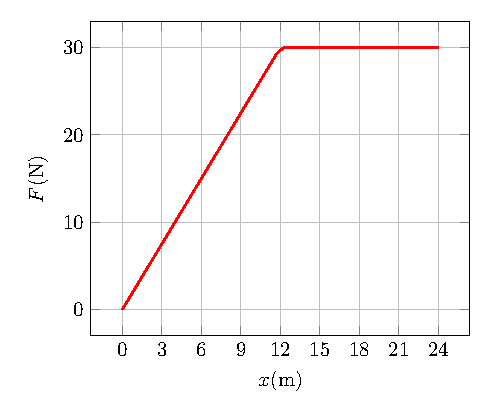
\includegraphics{hw-7-fig-1}
  \caption{Graph of the force $F$ with respect to distance.}
  \label{fig:hw-7-1}
\end{figure}
\end{problem}
\begin{proof}[Solution]
Remember that the work done by a force $F(x)$ over a distance
$a\leq x\leq b$ is given by the formula
\begin{equation}
  \label{eq:work}
W=\int_a^b F(x)\diff x.
\end{equation}
Since the graph in Figure (\ref{fig:hw-7-1}) is piecewise, all we need to
do is break up our interval $0\leq x\leq 24$ into the part where $y$ is a
diagonal line and where $y$ is a horizontal line, compute the work done on
each interval, $W_1$ and $W_2$, and add them up to get the total work
$W=W_1+W_2$.  First, note that over $0\leq x\leq 12$,
$F(x)=\frac{30}{12}x=\frac{5}{2}x$ so the work done from $0\leq x\leq 12$
is
\[
W_1=\int_0^{12}\frac{5}{2}x\diff x=
\left.\frac{5}{4}x^2\right|_0^{12}=
\frac{5}{4}(12)^2=\SI{180}{\joule}.
\]
Next, we see that $F(x)=30$ is constant for all $12\leq x\leq 24$
so we have
\[
W_2=\int_{12}^{24}F(x)\diff x=
\int_{12}^{24}30\diff x=
\left.30x\right|_{12}^{24}=
30\cdot 24-30\cdot 12=30\cdot 12=\SI{360}{\joule}.
\]
Hence, the total work done by $F(x)$ over $0\leq x\leq 24$ is
\[
  \boxed{W=W_1+W_2=\SI{180}{\joule}+\SI{360}{\joule}=\SI{540}{\joule}.}
\]
\end{proof}
\begin{problem}[WebAssign, HW8, 3]
A force of $6$ lb is required to hold a spring stretched $8$ in beyond its
natural length. How much work $W$ is done in stretching it from its natural
length to $14$ in beyond its natural length?
\end{problem}
\begin{proof}[Solution]
Recall \href{https://en.wikipedia.org/wiki/Hooke's_law}{Hooke's law} for
the force required to stretch a spring a distance $x$  beyond its natural
length
\begin{equation}
\label{eq:hookes-law}
F(x)=kx.
\end{equation}
Now, we are given a force of $6$ lb and a distance of $8$ in. Using this
information, we can figure out what the coefficient $k$ must be:
\[
k=F/x=6/8\mathrm{lb}/\mathrm{in}.
\]
Using the Equation (\ref{eq:work}) for work, we have that the work done on
a spring by stretching it from $x_1$ to $x_2$ is
\begin{equation}
\label{eq:work-on-spring}
W(x_1,x_2)=\int_{x_1}^{x_2}F(x)\diff x=\int_{x_1}^{x_2}kx\diff x=\left.\frac{1}{2}kx^2\right|_{x_1}^{x_2}=\frac{1}{2}k\left({x_1}^2-{x_2}^2\right)
\end{equation}
so, plugging in $14$, into our equation $W(x')$ above we get
\[
W(14)=\frac{1}{2}\cdot \frac{6}{8}\cdot
14^2=7\cdot\frac{6}{8}=\boxed{\frac{49}{8}\text{ ft-lb}.}
\]
\end{proof}
\begin{problem}[WebAssign, HW8, 4]
If the work required to stretch a spring $3$ ft beyond its natural length is
$9$ ft-lb, how much work is needed to stretch it $9$ in beyond its natural
length?
\end{problem}
\begin{proof}[Solution]
We employ the same idea as the one we used to calculate the work on the
last problem. First, we find the coefficient $k$, wit the help of Equation
(\ref{eq:work-on-spring}) this value will be
\[
k=\frac{2W}{x^2}=\frac{2\cdot 9}{9}=2\text{ lb}/\text{ft}.
\]
Now, convert our $9\text{ in}$ to ft we get $3/4\text{ ft}$. Lastly,
applying Equation (\ref{eq:work-on-spring}) on $3/4\text{ ft}$ we get
\[
W(3/4)=\frac{1}{2}\cdot 2\cdot (3/4)^2=\boxed{\frac{9}{16}\text{ in-lb}.}
\]
\end{proof}
\begin{problem}[WebAssign, HW8, 5]
An aquarium $\SI{6}{\meter}$ long, $\SI{1}{\meter}$ wide, and
$\SI{1}{\meter}$ deep is full of water. Find the work needed to pump half
of the water out of the aquarium. (Use $\SI{9.8}{\meter/\second^2}$ for $g$
and the fact that the density of water is
$\SI{1000}{\kilo\gram/\meter^3}$.)
\begin{itemize}
\item Show how to approximate the required work by a Riemann sum. (Let $x$
  be the height in meters below the top of the tank. Enter $x_i^*$ as $x_i$.)
\item Express the work as an integral.
\end{itemize}
\end{problem}
\begin{proof}[Solution]
Let's place the origin at the top of the tank. Then, the expression for the
work required to pump out half the water from our tank will be given
approximately by
\[
W(x)\approx\lim_{n\to\infty}\sum_{i=1}^n9.8\cdot1000\cdot 6\cdot x_i\Delta
x=\boxed{\sum_{i=1}^{n}58800 x_i^*\Delta x.}
\]
\\\\
Now we compute the integral from $0\leq x\leq 1/2$. We have
\[
W=58800\int_0^{1/2} x\diff x=5800\left(\left.\frac{1}{2}x^2\right|_0^{1/2} \right)=29400\left((1/2)^2-0\right)=\boxed{\SI{7350}{\joule}.}
\]
\end{proof}

\begin{problem}[WebAssign, HW8, 6]
A tank is full of water (see Figure \ref{fig:hw-7-2}). Find the work $W$
required to pump the water out of the spout. (Use
$\SI{9.8}{\meter/\second^2}$ for $g$. Use $\SI{1000}{\kilo\gram/\meter^3}$
as the weight density  of water. Assume that $a=\SI{4}{\meter}$,
$b=\SI{4}{\meter}$, $c=\SI{12}{\meter}$, and $d=\SI{2}{\meter}$.)
\begin{figure}[htbp]
  \centering
  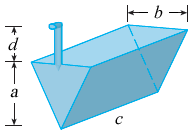
\includegraphics[scale=0.45]{hw-7-fig-2}
  \caption{A sketch of the tank.}
  \label{fig:hw-7-2}
\end{figure}
\end{problem}
\begin{proof}[Solution]
The work required to pump the water out of the spout of a tank with the
dimensions above is given by the
\[
W=\lim_{n\to\infty}\sum_{i=0}^n F(x_i)\Delta x
\]
where $\SI{0}{\meter}\leq x\leq\SI{8}{\meter}$. Now, the first thing we
need to do is to find the way the force changes as we move up the tank. Let
$x$ be the vertical distance from the bottom of the tank and $y$ be the
horizontal distance from. Then, the work needed to lift the slice slice of
volume $\Delta V$ that is a distance $(4+2)-x$ from the spout is
\begin{equation}
\label{eq:weight-density}
W(x)\approx g\rho(6-x)\Delta V,
\end{equation}
where $\rho$ is the density of the water and $g$ is gravity. Now, how does
our little slice of volume change as we move up the tank? If $y$ is the
side of the right-triangle made by going up a distance $x$ up the tank, then
\[
\frac{x}{y}=\frac{4}{4}=1
\]
since the triangles are similar. Hence, $y=2x$ so the volume change will be
\[
V(x)\approx 12\cdot\frac{1}{2}(2x)\Delta x=12x\Delta x(6-x),
\]
this is just the area of a triangle $x\Delta x$ (base times height) times
the depth $\SI{12}{\meter}$. Hence, the, plugging in the last equation into
our equation for the force (Equation (\ref{eq:weight-density})) will be
\[
W(x)\approx g\rho(6-x)\left(12 x\Delta x\right)=117600(6-x)x\Delta x
\]
Last but not least, we compute the limit as
$n\to\infty$,
\begin{align*}
W&=\lim_{n\to\infty}\sum_{i=0}^n W(x_i)\Delta x\\
\shortintertext{this is just the integral}
 &=117600\int_0^4(6-x)x\diff x\\
 &=117600\int_0^46x-x^2\diff x\\
 &=117600\left(\left.3x^2-\frac{1}{3}x^3\right|_0^4\right)\\
 &=117600\left(3\cdot 4^2-\frac{4^3}{3}-(0-0)\right)\\
 &=117600\left(\frac{3\cdot 3\cdot 4^2-4^3}{3}\right)\\
 &=117600\left(4^2\cdot\frac{9-4}{3}\right)\\
 &=117600\left(4^2\cdot\frac{5}{3}\right)\\
 &=\boxed{\SI{3136000}{\joule}.}
\end{align*}
\end{proof}
% p453:11,14
\begin{problem}[WebAssign, HW8, 7]
Consider the given function and the given interval
\[
f(x)=10\sin x-5\sin 2x,\quad[0,\pi]
\]
\begin{enumerate}[label=(\alph*)]
\item Find the average value $f_{\text{ave}}$ of $f$ on the given
  interval.
\item Find $c$ such that $f_{\text{ave}}=f(c)$.
\item Sketch the graph of $f$ and a rectangle whose area is the same as the
  area under the graph of $f$.
\end{enumerate}
\end{problem}
\begin{proof}[Solution]
(a) Recall the definition of the average of a function over an interval
$[a,b]$, it is
\begin{equation}
  \label{eq:average}
f_{\text{ave}}=\frac{1}{b-a}\int_a^b f\diff x.
\end{equation}
Now, all we need to do is calculate the integral of our $f$ and divide that
value by $\pi-0$, i.e.,
\begingroup
\allowdisplaybreaks
\begin{align*}
f_{\text{ave}}&=\frac{1}{\pi}\int_0^\pi f(x)\diff x\\
&=\frac{1}{\pi}\int_0^\pi 10\sin x-5\sin 2x\diff x\\
&=\frac{1}{\pi}\left(\left.-10\cos x+\frac{5}{2}\cos
  2x\right|_0^\pi\right)\\
&=\frac{1}{\pi}\left(-10\cos\pi+\frac{5}{2}\cos 2\pi-\left(-10\cos
  0+\frac{5}{2}\cos 0\right)\right)\\
&=\frac{1}{\pi}\left(10+\frac{5}{2}+10-\frac{5}{2}\right)\\
&=\frac{1}{\pi}\cdot 20\\
&=\boxed{\frac{20}{\pi}.}
\end{align*}
\endgroup
\\\\
(b) For this part all we need to do is set the equation $f(x)=10\sin
x-5\sin 2x$ equal to $20/\pi$ and solve for $x$:
\[
10\sin x-5\sin 2x=5(2\sin x-\sin 2x)=\frac{20}{\pi}
\]
so
\[
  2\sin x-\sin 2x=\frac{4}{\pi}.
\]
I can't think of any way to solve this than plugging it into your
calculator and having your calculator approximate the solution (your
calculator probably uses
\href{https://en.wikipedia.org/wiki/Newton's_method}{Newton's method},
which you will learn about later in your career). The values are about
\ul{$c\approx 1.238$ and $2.808$.}
\\\\
(c) Sketching the graph is easy and the box having the same area as will
have height equal to $20/\pi$ and length $\pi$. Multiply these together and
we get the area under the curve, which we computed to be $20$.
\end{proof}
\begin{problem}[WebAssign, HW8, 8]
Find the numbers b such that the average value of
$f(x)=7+10x-9x^2$ on the interval $[0,b]$ is equal to $8$.
\end{problem}
\begin{proof}[Solution]
This exercise is easy-peasy :-). All you need to do is compute the average
\[
f_\text{ave}=\frac{1}{b-0}\int_0^b7+10x-9x^2\diff x=7+5b-3b^2.
\]
Now, set the above equal to $8$ and we have
\[
7+5b-3b^2=8
\]
and solve for $b$. We get \ul{$b=(5-\sqrt{13})/6$ or $(5+\sqrt{13})/6$.}
\end{proof}

%%% Local Variables:
%%% mode: latex
%%% TeX-master: "../MA166-HW-Current"
%%% End:

\chapter{Homework 7 Solutions}

%%% Local Variables:
%%% mode: latex
%%% TeX-master: "../MA166-HW-Current"
%%% End:

\chapter{Homework 10 Solutions}
\begin{problem}[WebAssign HW 10, 1]
Evaluate the integral. (Use $C$ for the constant of integration.)
\[
\int 2\sin^2 x\cos^3 x\diff x
\]
\end{problem}
\begin{proof}[Solution]
First, note that $\cos^2 x=1-\sin^2 x$ so the integral above can be written
as
\begin{align*}
\int 2\sin^2 x\cos^3 x\diff x
&=\int 2\sin^2 x\cos^2 x\cos x\diff x\\
&=\int 2\sin^2x(1-\sin^2 x)\cos x\diff x.
\end{align*}
Now, make the substitution $u=\sin x$. Then $\diff u=\cos x\diff x$ so our
integral is now
\begin{align*}
\int 2u^2(1-u^2)\cos x\frac{\diff u}{\cos x}
&=\int 2u^2(1-u^2)\diff u\\
&=\int 2u^2-2u^4\diff u\\
&=\tfrac{2}{3}u^3-\tfrac{2}{5}u^5+C\\
&=\boxed{\tfrac{2}{3}\sin^3 x-\tfrac{2}{5}\sin^5 x+C.}
\end{align*}
\end{proof}

\begin{problem}[WebAssign HW 10, 2]
Evaluate the integral
\[
\int_0^{\pi/2}5\cos^2\theta\diff\theta.
\]
\end{problem}
\begin{proof}[Solution]
For this problem, we can use the double-angle identity, i.e.,
\begin{equation}
  \label{eq:cosine-double-angle}
\cos 2\theta=2\cos^2\theta-1=1-2\sin^2 x
\end{equation}
Substituting Equation (\ref{eq:cosine-double-angle}) into our integral, we
have
\begin{align*}
\int_0^{\pi/2}5\cos^2\theta\diff\theta&=
\int_0^{\pi/2}\tfrac{5}{2}(1+\cos 2\theta)\diff\theta\\
&=\tfrac{5}{2}\int_0^{\pi/2}(1+\cos 2\theta)\diff\theta\\
&=\tfrac{5}{2}\left(\left.\theta+\tfrac{1}{2}\sin
  2\theta\right|_0^{\pi/2}\right)\\
&=\tfrac{5}{2}\left(\frac{\pi}{2}+0-(0+0)\right)\\
&=\boxed{\frac{5\pi}{4}.}
\end{align*}
\end{proof}

\begin{problem}[WebAssign HW 10, 3]
Evaluate the integral.
\[
\int_0^{\pi/2}5\sin^2 x\cos^2 x\diff x.
\]
\end{problem}
\begin{proof}[Solution]
Again, we just use a trigonometric identity, specifically
\begin{equation}
  \label{eq:sine-double-angle}
\sin 2 x =2\sin  x \cos x .
\end{equation}
Using Equation (\ref{eq:sine-double-angle}) our integral turns into
\begin{align*}
\int_0^{\pi/2}5\sin^2x\cos^2x\diff x
&=5\int_0^{\pi/2}\tfrac{1}{4}(4\sin^2 x\cos^2x)\diff x\\
&=\frac{5}{4}\int_0^{\pi/2}(2\sin x\cos x)^2\diff x\\
&=\frac{5}{4}\int_0^{\pi/2}(\sin 2x)^2\diff x\\
&=\frac{5}{4}\int_0^{\pi/2}\sin^2 2x\diff x\\
&=\frac{5}{4}\int_0^{\pi/2}\sin^2 2x\diff x\\
\shortintertext{now we use this identity $2\sin^2 x =1-\cos 2 x $
  to get}
&=\frac{5}{4}\int_0^{\pi/2}\frac{1}{2}(1-\cos 4 x )\diff x \\
&=\frac{5}{8}\int_0^{\pi/2}1-\cos 4 x \diff x \\
&=\frac{5}{8}\left(\left. x -\tfrac{1}{4}\sin
  4 x \right|_0^{\pi/2}\right)\\
&=\boxed{\tfrac{5\pi}{16}.}
\end{align*}
\end{proof}

\begin{problem}[WebAssign HW 10, 4]
Evaluate the integral. (Remember to use $\ln(|u|)$ where appropriate. Use
$C$ for constant of integration.)
\[
\int 9\cos^2 x\tan^3 x\diff x.
\]
\end{problem}
\begin{proof}[Solution]
Let's make the substitution $u=\cos x$ so $\diff u=-\sin x\diff x$ and we
have
\begingroup
\allowdisplaybreaks
\begin{align*}
\int 9\cos^2 x\tan^3 x\diff x
&=9\int \cos^2 x\tan^3 x\diff x\\
&=9\int\frac{\cos^2 x\sin^3 x}{\cos^3 x}\diff x\\
&=9\int\frac{\sin^3 x}{\cos x}\diff x\\
&=9\int\frac{\sin x(1-\cos^2 x)}{\cos x}\diff x\\
\shortintertext{now, for the substitution,}
&=9\int\frac{\sin x(1-u^2)}{u}\frac{\diff u}{-\sin x}\\
&=9\int\frac{u^2-1}{u}\diff u\\
&=9\int u-\frac{1}{u}\diff u\\
&=\tfrac{9}{2}u^2-9\ln|u|+C\\
\shortintertext{and back, we have}
&=\boxed{\tfrac{9}{2}\cos^2 x-9\ln|\cos x|+C.}
\end{align*}
\endgroup
\end{proof}

\begin{problem}[WebAssign HW 10, 5]
Evaluate the integral. (Use $C$ for the constant of integration.)
\[
\int 5\tan^2 x\diff x.
\]
\end{problem}
\begin{proof}[Solution]
The easiest one so far. Recall the identity
\begin{equation}
  \label{eq:tangent-identity}
\sec^2 x -\tan^2 x =1.
\end{equation}
Then, we gave
\[
\int 5\tan^2x\diff x=5\int(\sec^2 x -1)\diff x =
\boxed{5\tan x -5 x +C.}
\]
\end{proof}

% p476:1,7,11,17,23,24,35,61
\begin{problem}[WebAssign HW 10, 6]
\[
\int 8\left(\tan^2x+\tan^4x\right)\diff x.
\]
\end{problem}
\begin{proof}[Solution]
We'll make the substitution $u=\tan x$, so $\diff u=\sec^2x\diff
x$. Proceeding, we have
\begin{align*}
\int 8\left(\tan^2 x+\tan^4x\right)\diff x
&=8\int\tan^2 x(1+\tan^2 x)\diff x\\
\shortintertext{by Equation (\ref{eq:tangent-identity}), we have}
&=8\int\tan^2 x\sec^2 x\diff x\\
&=8\int u^2\diff u\\
&=\tfrac{8}{3}u^3+C\\
&=\boxed{\tfrac{8}{3}\tan^3 x+C.}
\end{align*}
\end{proof}

\begin{problem}[WebAssign HW 10, 7]
Evaluate the integral
\[
\int_{\pi/6}^{\pi/2}\cot^2 x\diff x
\]
\end{problem}
\begin{proof}[Solution]
Remember that, like Equation (\ref{eq:tangent-identity}), there is a
cotangent-identity
\begin{equation}
  \label{eq:cotangent-identity}
1+\cot^2 x=\csc^2 x.
\end{equation}
With the help of this equation, we have
\begin{align*}
\int_{\pi/6}^{\pi/2}\cot^2 x\diff x&=
\int_{\pi/6}^{\pi/2}(\csc^2-1)\diff x\\
&=\left.-\cot x-x\right|_{\pi/6}^{\pi/2}\\
&=0-\frac{\pi}{2}-\left(\sqrt{3}-\frac{\pi}{6}\right)\\
&=\boxed{\sqrt{3}-\frac{\pi}{3}.}
\end{align*}
\end{proof}

\begin{problem}[WebAssign HW 10, 8]
Find the volume $V$ obtained by rotating the region bounded by the given
curves about the specified axis.
\[
y=9\sin x,\quad
y=0,\quad
\frac{\pi}{2}\leq x\leq\pi;\qquad
\text{about the $x$-axis.}
\]
\end{problem}
\begin{proof}[Solution]
Since we are rotating about the $x$-axis, we need to find the
cross-sectional area in terms of $y$ in terms of $x$, hence we have
\[
A(x)=\pi y^2=81\pi\sin^2 x.
\]
Now, integrating from $\pi/2$ to $\pi$, we get
\begin{align*}
\int_{\pi/2}^\pi A(x)\diff x
&=81\pi\int_{\pi/2}^\pi \sin^2 x\\
\shortintertext{using the double-angle identity for cosine, Equation
  (\ref{eq:cosine-double-angle}), we get}
&=81\pi\int_{\pi/2}^\pi \tfrac{1}{2}(1-\cos 2x)\diff x\\
&=\tfrac{81\pi}{2}\left(\left.x-\tfrac{1}{2}\sin 2x\right|_{\pi/2}^\pi\right)\\
&=\tfrac{81\pi}{2}\left(\pi-0-(\tfrac{1}{2}\pi)\right)\\
&=\boxed{\frac{81\pi^2}{4}.}
\end{align*}
\end{proof}

%%% Local Variables:
%%% mode: latex
%%% TeX-master: "../MA166-HW-Current"
%%% End:

%%% Local Variables:
%%% mode: latex
%%% TeX-master: "../MA166-Recitation"
%%% End:

\end{document}

%%% Local Variables:
%%% mode: latex
%%% TeX-master: t
%%% End:
